\section{SOFTWARE}

\subsection{Implantação}

O sistema é composto por duas aplicações independentes implantadas na plataforma Render, a partir de dois repositórios no GitHub: frontend (\url{https://github.com/igordev23/certificate-hub}) e backend (\url{https://github.com/igordev23/Certificate-server}). O sistema é publicado sob subdomínios automáticos fornecidos pela plataforma, garantindo tráfego criptografado via SSL/HTTPS de forma nativa. O frontend pode ser acessado, por exemplo, em \url{https://certificate-hub.onrender.com}, enquanto a API do backend responde em \url{https://certificate-server-zd0m.onrender.com}.

\subsubsection{Arquitetura e Execução}

Para a execução e construção do projeto, é estipulado o uso do Node.js, configurado no Render através da variável de ambiente \texttt{NODE\_VERSION}. A implantação distingue a arquitetura das duas aplicações:

\begin{itemize}
    \item \textbf{Frontend (Static Site):} Trata-se de uma \textit{Single Page Application} (SPA) em Vite. O serviço de \textit{Static Site} serve exclusivamente arquivos estáticos (HTML, CSS e JavaScript gerados na pasta \texttt{dist}) diretamente, sem manter um processo de execução ativo (\textit{runtime} Node). O roteamento no lado do cliente é delegado ao TanStack Router via \textit{History API}.
    \item \textbf{Backend (Web Service):} Construído em Next.js (utilizando recursos de servidor Node.js), opera como um \textit{Web Service}, ou seja, mantém um processo vivo que processa requisições HTTP dinâmicas em tempo real. O processo de implantação exige a execução do comando de compilação (\texttt{npm run build}) antes da inicialização do servidor com \texttt{npm start}.
\end{itemize}

\subsubsection{CI/CD e Pipeline de Implantação}

O fluxo de implantação baseia-se em um pipeline de CI/CD (Integração e Entrega Contínuas). A etapa de \textit{Continuous Integration} (CI) é gerenciada pelo GitHub Actions, que executa automaticamente as suítes de testes a cada \textit{push} na branch \texttt{main}. Se os testes passarem com sucesso, a etapa de \textit{Continuous Deployment} (CD) é acionada no Render, que compila e publica a nova versão. Em caso de falha nos testes (no GitHub Actions) ou no \textit{build} (no Render), o processo é interrompido, impedindo que código defeituoso chegue a produção. Caso um comportamento inesperado ocorra pós-deploy, a plataforma fornece uma estratégia simples de \textit{rollback}, permitindo reverter imediatamente para o \textit{deploy} anterior funcional com um único clique. A Figura~\ref{fig:deploy} ilustra o fluxo.

\begin{figure}[H]
\centering
\caption{Pipeline de CI do backend no GitHub Actions}
\label{fig:ci-backend}
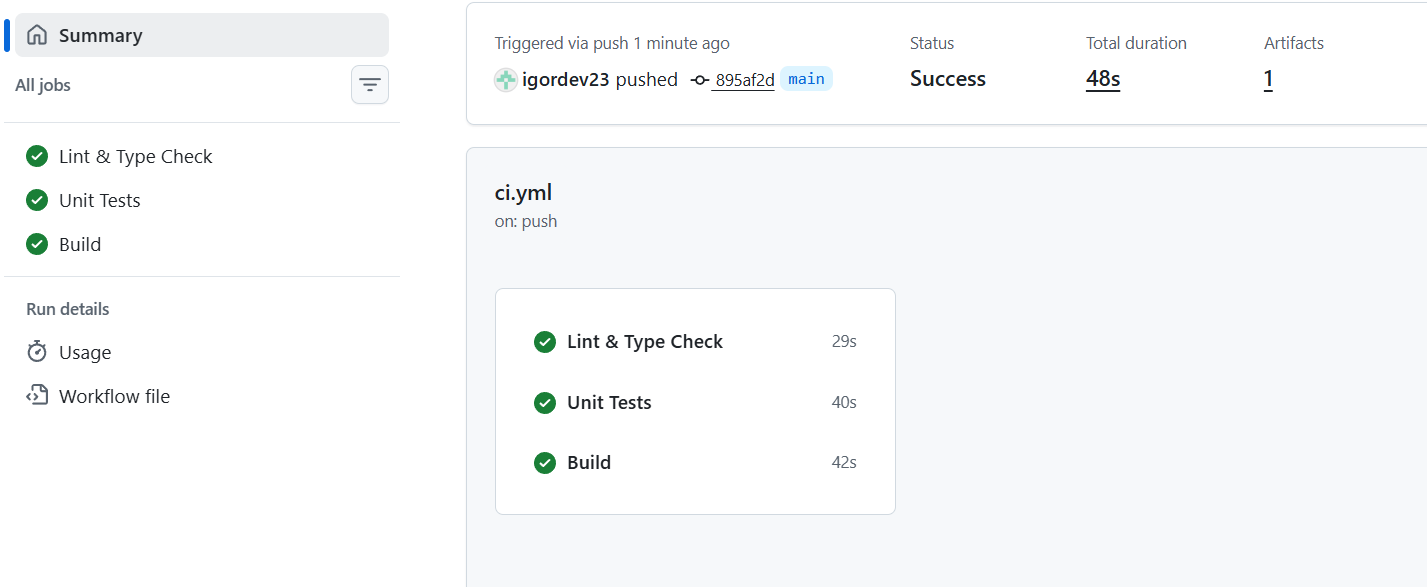
\includegraphics[width=\textwidth]{imagens/CIbackend.png}
\par\vspace{0.5em}
\parbox{\textwidth}{\raggedright\small\textit{Fonte: Elaborado pelo Autor (2026).}}
\end{figure}

\begin{figure}[H]
\centering
\caption{Pipeline de CI do frontend no GitHub Actions}
\label{fig:ci-frontend}
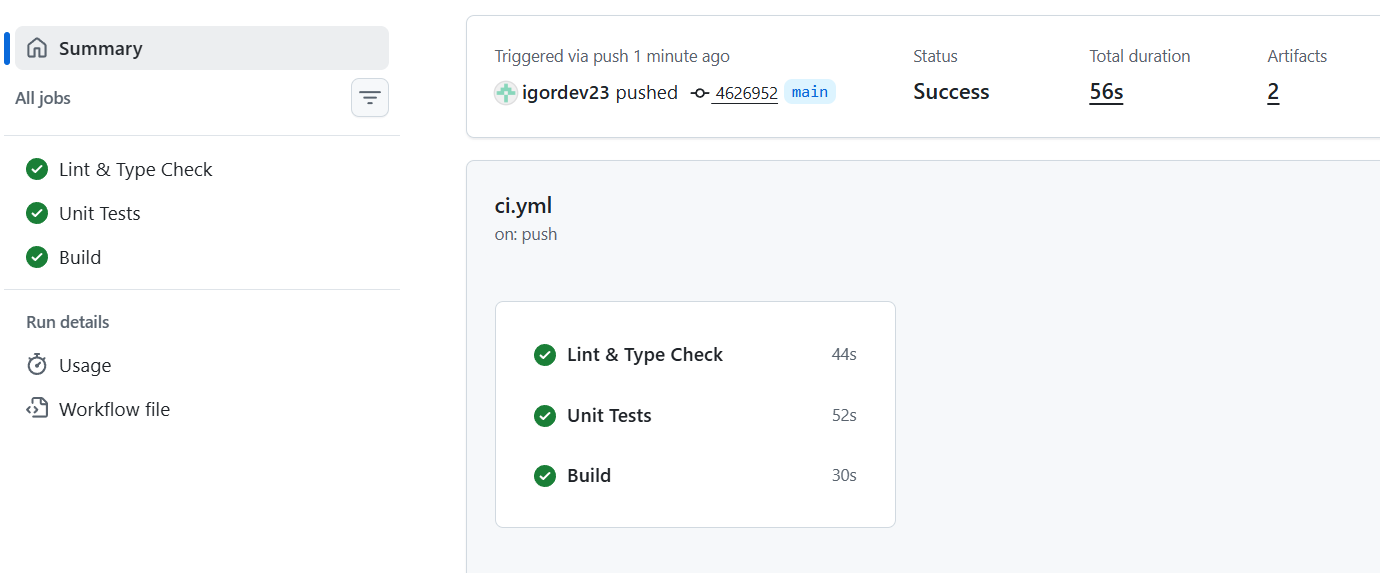
\includegraphics[width=\textwidth]{imagens/CIfrontend.png}
\par\vspace{0.5em}
\parbox{\textwidth}{\raggedright\small\textit{Fonte: Elaborado pelo Autor (2026).}}
\end{figure}

\subsubsection{Configuração de Ambiente}

Para assegurar o isolamento das configurações sensíveis, utilizam-se variáveis de ambiente não expostas no código. Os modelos de configuração adotados incluem:

\begin{itemize}
    \item \textbf{Frontend:} \texttt{VITE\_API\_URL} (aponta para a URL do Web Service backend).
    \item \textbf{Backend:}
    \begin{itemize}
        \item \texttt{DATABASE\_URL} (string de conexão PostgreSQL);
        \item \texttt{NEXT\_PUBLIC\_SUPABASE\_URL} (URL do projeto Supabase);
        \item \texttt{NEXT\_PUBLIC\_SUPABASE\_PUBLISHABLE\_KEY} (chave pública do Supabase);
        \item \texttt{NEXT\_PUBLIC\_FRONTEND\_URL} (URL do frontend para configuração de CORS).
    \end{itemize}
\end{itemize}

\subsubsection{Banco de Dados}

O armazenamento é delegado ao PostgreSQL hospedado via Supabase. O banco de dados utiliza \textit{connection pooling} nativo (gerenciamento de conexões otimizado) para alta concorrência e conta com política de backup automático gerida pela plataforma. As atualizações estruturais (\textit{schema}) são aplicadas através de migrações executadas automaticamente na fase de \textit{build}.

\subsubsection{Monitoramento e Observabilidade}

Por fim, a observabilidade do sistema e o monitoramento (\textit{health checks}) são garantidos pelos logs em tempo real nativos do Render, permitindo diagnóstico ágil de eventuais gargalos de desempenho e verificação de saúde da aplicação.

\begin{figure}[H]
    \centering
    \caption{Diagrama de Implantação — Fluxo de deploy no Render a partir do GitHub, com frontend como Static Site, backend como Web Service e banco PostgreSQL gerenciado pelo Supabase}
    \label{fig:deploy}
    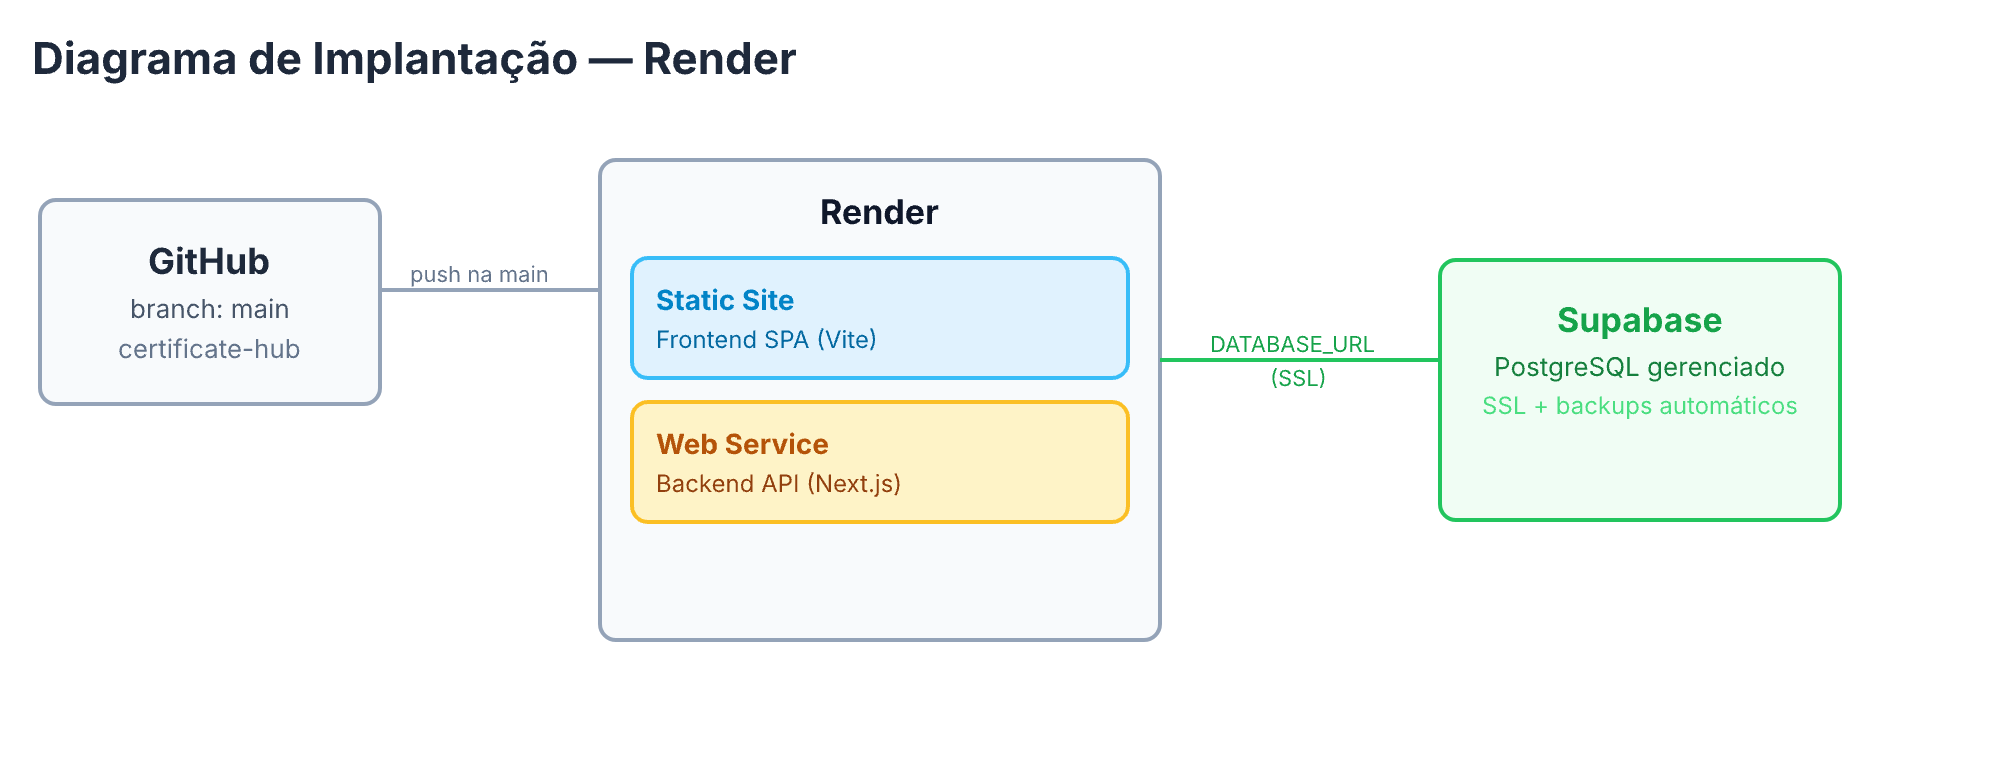
\includegraphics[width=0.85\textwidth]{imagens/deploy.png}
    \par\vspace{0.5em}
    \parbox{\textwidth}{\raggedright\small\textit{Fonte: Elaborado pelo Autor (2026).}}
\end{figure}


\subsection{Exemplos de Código}
\label{sec:exemplos-codigo}

Esta seção apresenta trechos reais do código-fonte do sistema que ilustram as principais funcionalidades implementadas. Os exemplos foram extraídos do backend (CertifyHub Server), construído com Next.js e TypeScript seguindo os princípios de arquitetura limpa.

\subsubsection{Entidade de Domínio: Certificate}
\label{sec:codigo-certificate}

O Código~\ref{cod:certificate} apresenta a entidade \code{Certificate}, que encapsula as regras de negócio relacionadas à emissão e validação de certificados. A classe utiliza um construtor privado e métodos estáticos de fábrica (\code{create} e \code{fromPersistence}) para garantir que apenas instâncias válidas sejam criadas. O método \code{isValid()} (linha~\ref{line:isvalid}) implementa a regra de negócio que determina se um certificado está dentro do prazo de validade, comparando a data de validade com a data atual.

\begin{lstlisting}[language=TypeScript, caption={Entidade Certificate com validações de domínio}, label={cod:certificate}, escapechar=§]
export class Certificate {
  private constructor(private props: CertificateProps) {}

  static create(props: Omit<CertificateProps, "createdAt" | "updatedAt">): Certificate {
    Certificate.validate(props);
    return new Certificate({ ...props, createdAt: new Date(), updatedAt: new Date() });
  }

  static fromPersistence(props: CertificateProps): Certificate {
    return new Certificate({ ...props, validityDate: new Date(props.validityDate) });
  }

  isValid(): boolean {       §\label{line:isvalid}§
    return this.props.validityDate > new Date();
  }

  updateValidity(newDate: Date): void {
    if (newDate <= new Date()) throw new InvalidValidityDateError();
    this.props.validityDate = newDate;
    this.props.updatedAt = new Date();
  }

  private static validate(props: Omit<CertificateProps, "createdAt" | "updatedAt">): void {
    if (!props.recipientName?.trim()) throw new InvalidCertificateDataError("Nome é obrigatório");
    if (!props.recipientCPF || props.recipientCPF.length !== 11)
      throw new InvalidCertificateDataError("CPF deve ter 11 dígitos");
    if (!props.courseHours || props.courseHours <= 0)
      throw new InvalidCertificateDataError("Carga horária deve ser maior que zero");
    if (!props.templateId) throw new InvalidCertificateDataError("Template é obrigatório");
  }
}
\end{lstlisting}
\noindent\raggedright\small\textit{Fonte: Elaborado pelo Autor (2026).}

\subsubsection{Route Handler de Emissão}
\label{sec:codigo-emissao}

O Código~\ref{cod:emit} mostra o \textit{Route Handler} responsável pela emissão de certificados (\ref{rf:gerar-pdf}). A requisição \code{POST /api/certificates/emit} recebe os dados do certificado, valida-os com Zod (\code{emitCertificateSchema.parse}), instancia os repositórios concretos e delega a execução ao caso de uso \code{EmitCertificateUseCase}. O uso de injeção de dependência nos repositórios (linhas~\ref{line:repos} e~\ref{line:repos2}) permite substituir as implementações sem alterar a lógica de negócio.

\begin{lstlisting}[language=TypeScript, caption={Route Handler de emissão de certificado}, label={cod:emit}, escapechar=§]
export async function POST(request: Request) {
  try {
    const body = await request.json();
    const validated = emitCertificateSchema.parse(body);

    const certificateRepo = new SupabaseCertificateRepository();§\label{line:repos}§
    const templateRepo = new SupabaseTemplateRepository();§\label{line:repos2}§
    const useCase = new EmitCertificateUseCase(certificateRepo, templateRepo);

    const { certificate } = await useCase.execute(validated);

    return NextResponse.json(
      { data: certificate.toJSON(), message: "Certificado emitido com sucesso" },
      { status: 201 }
    );
  } catch (error) {
    return handleApiError(error);
  }
}
\end{lstlisting}
\noindent\raggedright\small\textit{Fonte: Elaborado pelo Autor (2026).}

\subsubsection{Geração de PDF com \textit{QR Code}}
\label{sec:codigo-pdf}

O Código~\ref{cod:pdf} apresenta o serviço \code{PDFKitService} que gera o PDF do certificado com \textit{QR Code} de verificação (\ref{rf:qrcode}). A URL de verificação é montada a partir da variável de ambiente \code{NEXT\_PUBLIC\_VERIFY\_URL} (linha~\ref{line:verifyurl}) e codificada em um \textit{QR Code} utilizando a biblioteca \code{qrcode} (linha~\ref{line:qrcode}). A imagem gerada é inserida no PDF na posição inferior esquerda (linha~\ref{line:qrimage}), acompanhada das instruções de verificação e do código único.

\begin{lstlisting}[language=TypeScript, caption={Geração de PDF com QR Code no servidor}, label={cod:pdf}, escapechar=§]
const verifyUrl = `${process.env.NEXT_PUBLIC_VERIFY_URL ||§\label{line:verifyurl}§
  "https://example.com/verify"}?cpf=${certificate.recipientCPF}
  &codigo=${certificate.verificationCode}`;

const qrBuffer = await toBuffer(verifyUrl, {           §\label{line:qrcode}§
  width: 160, margin: 1,
  color: { dark: template.layoutConfig.primaryColor, light: "#ffffff" },
});

const doc = new PDFDocument({ layout: "landscape", size: "A4" });

// Posicionar QR Code no canto inferior esquerdo
doc.image(qrBuffer, 80, instrY, { width: 60 });        §\label{line:qrimage}§

// Instruções de verificação ao lado do QR Code
doc.font("Helvetica-Bold").fontSize(9).text(
  "INSTRUÇÕES PARA VERIFICAÇÃO DE AUTENTICIDADE:", instrX, instrY
);
doc.font("Helvetica").fontSize(8).text(
  \`Este certificado foi emitido pelo CertifyHub.
  Verifique a sua autenticidade acessando o QR Code...\`, instrX, instrY + 14
);
\end{lstlisting}
\noindent\raggedright\small\textit{Fonte: Elaborado pelo Autor (2026).}

\subsubsection{Validação por Código Único}
\label{sec:codigo-validacao}

O Código~\ref{cod:verify-handler} apresenta o \textit{Route Handler} público \code{POST /api/verify} que implementa a validação de autenticidade de certificados (\ref{rf:portal-validacao}--\ref{rf:exibir-validacao}). A requisição recebe o CPF e o código de verificação presentes no certificado, valida a entrada com Zod (\code{verifyCertificateSchema}) e delega a lógica ao \code{VerifyCertificateUseCase}.

\begin{lstlisting}[language=TypeScript, caption={Route Handler público de verificação de autenticidade}, label={cod:verify-handler}, escapechar=§]
export async function POST(request: Request) {
  try {
    const body = await request.json();
    const validated = verifyCertificateSchema.parse(body);

    const repo = new SupabaseCertificateRepository();
    const useCase = new VerifyCertificateUseCase(repo);
    const result = await useCase.execute(validated);

    return NextResponse.json({ data: result });
  } catch (error) {
    return handleApiError(error);
  }
}
\end{lstlisting}
\noindent\raggedright\small\textit{Fonte: Elaborado pelo Autor (2026).}

O Código~\ref{cod:verify-usecase} detalha o caso de uso \code{VerifyCertificateUseCase}, que centraliza a lógica de verificação. O método \code{execute} busca o certificado no banco por CPF e código (\ref{rf:validar-certificado}); se encontrado, retorna os dados do certificado e o status de validade calculado pelo método \code{isValid()} da entidade de domínio. Se não encontrado, indica que o certificado não é autêntico.

\begin{lstlisting}[language=TypeScript, caption={Caso de uso de verificação de autenticidade}, label={cod:verify-usecase}, escapechar=§]
export class VerifyCertificateUseCase {
  constructor(private readonly certificateRepo: ICertificateRepository) {}

  async execute(dto: VerifyCertificateDTO): Promise<VerifyCertificateResult> {
    const certificate = await this.certificateRepo.findByCPFAndCode(
      dto.cpf,
      dto.verificationCode.toUpperCase()
    );

    if (!certificate) {
      return { isAuthentic: false, isValid: false, certificate: null };
    }

    return {
      isAuthentic: true,
      isValid: certificate.isValid(),
      certificate: {
        recipientName: certificate.recipientName,
        courseName: certificate.courseName,
        courseHours: certificate.courseHours,
        issuedAt: certificate.issuedAt,
        validityDate: certificate.validityDate,
        verificationCode: certificate.verificationCode,
      },
    };
  }
}
\end{lstlisting}
\noindent\raggedright\small\textit{Fonte: Elaborado pelo Autor (2026).}

\subsection{Testes}

Conforme definido nos objetivos específicos da Seção~\ref{sec:objetivos-especificos}, foram planejados e executados testes unitários para validação dos módulos implementados no escopo do MVP. Os casos de teste foram elaborados com base nos critérios de aceitação apresentados no Quadro~\ref{qua:criterios} e abrangem os requisitos funcionais classificados como prioritários — \textit{Must have} [M] e \textit{Should have} [S] — essenciais para a primeira versão do sistema.

Os testes foram classificados como unitários, uma vez que cada módulo (frontend e backend) foi testado de forma isolada, com dependências externas (banco de dados, APIs de terceiros, bibliotecas de geração de PDF) substituídas por \textit{mocks}. Testes não-funcionais de carga, segurança (\textit{rate limiting} e autenticação) e acessibilidade foram implementados com escopo reduzido, conforme detalhado nas subseções seguintes. Testes de integração não foram incluídos no escopo do MVP, podendo ser abordados em versões futuras do sistema. Testes \textit{end-to-end} (E2E) foram implementados com Playwright para validar o fluxo completo do sistema, conforme descrito na Seção~\ref{subsubsec:e2e}. Todos os testes foram executados em ambiente local, com Node.js 22, e integraram o pipeline de CI/CD do Render, que executa a suíte completa a cada \textit{push} na branch \texttt{main}.

\subsubsection{Plano de Testes}

\paragraph{Estratégia de Testes}

O plano de testes foi elaborado com base nos requisitos funcionais (Seção~3.1.1) e nos critérios de aceitação (Quadro~\ref{qua:criterios}), contemplando exclusivamente os módulos implementados no escopo do MVP. A estratégia adotada prioriza testes unitários como primeira camada de defesa, combinada com testes de integração para validação das camadas de infraestrutura e testes \textit{end-to-end} (E2E) para verificação do fluxo completo do sistema.

\begin{itemize}
    \item \textbf{Ferramentas:} Jest como \textit{test runner} e \textit{framework} de asserção; React Testing Library para testes de \textit{ViewModels} no frontend; Playwright para testes \textit{end-to-end}; \textit{Mocking} manual via \texttt{jest.mock} para isolar dependências externas (Supabase, PDFKit, \texttt{fetch}).
    \item \textbf{Execução em CI/CD:} A suíte completa é executada automaticamente pelo Render a cada \textit{push} na branch \texttt{main}. O pipeline valida que todos os testes passem antes da implantação.
    \item \textbf{Meta de cobertura:} O projeto define cobertura mínima de 75\% em \textit{Statements}, \textit{Functions} e \textit{Lines}, configurada no Jest e validada no pipeline de CI. As camadas de domínio e casos de uso no backend têm meta informal de 100\%.
    \item \textbf{Massa de dados:} Os testes de repositório utilizam o cliente Supabase \textit{mockado}, dispensando banco de dados real. Para testes das entidades de domínio, os dados são construídos em memória (\textit{in-memory}), garantindo isolamento total entre cenários.
\end{itemize}

\paragraph{Casos de Teste}

Cada caso de teste é identificado por um código único (CT\textit{nnn}) e descreve o cenário avaliado juntamente com o resultado esperado. O Quadro~\ref{qua:plano-testes} apresenta o plano completo, organizado por módulo e tipo de teste.

\renewcommand{\arraystretch}{0.85}
\small
\begingroup
\renewcommand{\tablename}{Quadro}
\renewcommand{\LTcaptype}{quadro}
\begin{longtable}{p{1.2cm} p{4.2cm} p{7.5cm} p{2.6cm}}
\caption{Plano de testes do sistema}
\label{qua:plano-testes}\\
\toprule
\textbf{Caso} & \textbf{Descrição} & \textbf{Resultados Esperados} & \textbf{Status} \\
\midrule
\endfirsthead
\toprule
\textbf{Caso} & \textbf{Descrição} & \textbf{Resultados Esperados} & \textbf{Status} \\
\midrule
\endhead
\bottomrule
\endfoot
\bottomrule
\endlastfoot

\multicolumn{4}{l}{\textbf{Módulo de Templates de Certificados (\ref{rf:upload-templates}--\ref{rf:duplicar-templates})}} \\
\midrule

CT001 & Criação de template & Template é criado com nome, descrição e \textit{layout} mesclado aos valores padrão. & Executado \\
CT002 & Listagem de templates & \textit{Endpoint} retorna lista de templates cadastrados. & Executado \\
CT003 & Obtenção de template por ID & \textit{Endpoint} retorna template específico; lança erro \texttt{TemplateNotFoundError} se não existir. & Executado \\
CT004 & Edição de template & Nome, descrição e configurações de \textit{layout} são alterados e persistem. & Executado \\
CT005 & Exclusão de template & Template é removido após confirmação do usuário; \textit{endpoint} \texttt{delete} é chamado. & Executado \\
CT006 & Personalização de \textit{layout} & Configurações parciais são mescladas com os valores padrão (\texttt{DEFAULT\_LAYOUT}). & Executado \\

\midrule
\multicolumn{4}{l}{\textbf{Módulo de Geração de Certificados (\ref{rf:gerar-pdf}--\ref{rf:download-lote})}} \\
\midrule

CT007 & Emissão manual de certificado & Selecionar template, preencher dados e confirmar gera certificado com código único. & Executado \\
CT008 & Geração de PDF & PDF gerado preserva layout, cores e fontes do template; resultado é um \textit{Buffer} binário. & Executado \\
CT009 & Geração de PDF com cores personalizadas & PDF é gerado com \texttt{backgroundColor}, \texttt{primaryColor} e \texttt{borderColor} personalizados. & Executado \\
CT010 & Geração de PDF sem borda & PDF é gerado corretamente com \texttt{showBorder = false}. & Executado \\
CT011 & Erro na geração de PDF & Falha no PDFKit rejeita a \textit{Promise} com mensagem de erro. & Executado \\
CT012 & Obtenção de certificado por ID & \textit{Endpoint} retorna certificado específico; lança erro \texttt{CertificateNotFoundError} se não existir. & Executado \\
CT013 & Listagem de certificados & \textit{Endpoint} retorna lista de certificados cadastrados. & Executado \\
CT014 & Atualização de certificado & Nome, CPF, carga horária, curso e \texttt{templateId} são alterados individual ou simultaneamente. & Executado \\
CT015 & Atualização de validade & Data de validade é atualizada; data passada é rejeitada. & Executado \\
CT016 & Validação de dados de entrada & Nome vazio, CPF inválido, carga horária negativa e \texttt{templateId} não-UUID são rejeitados. & Executado \\
CT017 & Validação de CPF & CPF com dígitos verificadores incorretos ou todos iguais é rejeitado. & Executado \\
CT018 & Formatação de CPF & CPF é automaticamente formatado (XXX.XXX.XXX-XX) durante a digitação. & Executado \\
CT019 & Emissão com template inexistente & \textit{Endpoint} lança \texttt{TemplateNotFoundError} se o \texttt{templateId} não existir. & Executado \\

\midrule
\multicolumn{4}{l}{\textbf{Módulo de Validação Pública e Antifraude (\ref{rf:portal-validacao}--\ref{rf:exibir-validacao})}} \\
\midrule

CT020 & Validação via código único & Código válido retorna certificado com status autêntico e válido. & Executado \\
CT021 & Certificado expirado & Certificado com validade vencida é retornado como autêntico, porém inválido. & Executado \\
CT022 & Código não encontrado & Código inexistente é rejeitado e a validação retorna certificado não localizado. & Executado \\
CT023 & \textit{Case insensitive} na consulta & Código digitado em minúsculo é convertido para maiúsculo antes da consulta no banco. & Executado \\
CT024 & Remoção de máscara do CPF & CPF com pontuação tem os caracteres não numéricos removidos antes da consulta. & Executado \\
CT025 & Tratamento de erro na validação & Erros retornados pela API são exibidos ao usuário e o estado de carregamento é gerenciado corretamente. & Executado \\

\midrule
\multicolumn{4}{l}{\textbf{Módulo de \textit{Dashboard} e Gestão (\ref{rf:lista-certificados}--\ref{rf:estatisticas-emissao})}} \\
\midrule

CT026 & Listagem de certificados & Tabela exibe certificados carregados da API com gerenciamento do estado de carregamento. & Executado \\
CT027 & Filtro por nome, CPF e código & Digitar texto no campo de busca filtra a lista em tempo real. & Executado \\
CT028 & Cópia do código de verificação & Botão copia o código para a área de transferência. & Executado \\
CT029 & Atualização de validade na interface & Usuário altera data de validade; a requisição é enviada ao servidor e a lista é recarregada. & Executado \\
CT030 & Estatísticas do \textit{dashboard} & Painel exibe total de certificados, ativos, templates e envios. & Executado \\
CT031 & Cálculo de certificados ativos & Certificados expirados são excluídos da contagem de ativos. & Executado \\

\midrule
\multicolumn{3}{l}{\textbf{Entidades de Domínio}} \\
\midrule

CT032 & Criação de certificado válido & Entidade \texttt{Certificate} é criada com todos os campos obrigatórios. & Executado \\
CT033 & Validações da entidade Certificate & Nome vazio, CPF inválido, curso vazio, carga horária zero/negativa e \texttt{templateId} vazio disparam erro de domínio. & Executado \\
CT034 & Data de validade futura & Certificado com validade futura retorna \texttt{isValid = true}. & Executado \\
CT035 & Data de validade passada & Certificado com validade passada retorna \texttt{isValid = false}. & Executado \\
CT036 & Criação de template válido & Entidade \texttt{Template} é criada com \textit{layout} mesclado aos valores \textit{default}. & Executado \\
CT037 & Validações da entidade Template & Nome vazio ou com apenas espaços dispara erro de domínio. & Executado \\
CT038 & Geração de código de verificação & Código gerado possui exatamente 8 caracteres do \textit{charset} definido. & Executado \\
CT039 & Comparação de códigos & Método \texttt{equals()} compara dois códigos corretamente; \textit{case insensitive}. & Executado \\
CT040 & Erros de domínio & Classes de erro (\texttt{CertificateNotFoundError}, \texttt{InvalidCPFError}, etc.) possuem mensagens e \textit{status} HTTP adequados. & Executado \\
CT041 & Restauração a partir de persistência & Dados vindos do banco são convertidos corretamente para instâncias das entidades. & Executado \\

\midrule
\multicolumn{3}{l}{\textbf{Camada de Infraestrutura}} \\
\midrule

CT042 & Repositório de certificados — consultas & Operações \texttt{findById}, \texttt{findByCPFAndCode} e \texttt{findAll} retornam certificados ou \texttt{null}. & Executado \\
CT043 & Repositório de certificados — escrita & Operações \texttt{create}, \texttt{update} e \texttt{delete} persistem no Supabase e tratam erros. & Executado \\
CT044 & Repositório de templates — consultas & Operações \texttt{findById} e \texttt{findAll} retornam templates ou \texttt{null} com \textit{fallback} de valores. & Executado \\
CT045 & Repositório de templates — escrita & Operações \texttt{create}, \texttt{update} e \texttt{delete} persistem no Supabase e tratam erros. & Executado \\
CT046 & Geração de PDF com PDFKit & PDF é gerado como \textit{Buffer}; cores e bordas são aplicadas; erro no PDFKit é tratado. & Executado \\
CT047 & Tratamento de erros da API & Erros de domínio (404, 400), erros Zod (400) e erros inesperados (500) são mapeados para \textit{status code} HTTP corretos. & Executado \\

\midrule
\multicolumn{3}{l}{\textbf{Utilitários (\textit{Frontend})}} \\
\midrule

CT048 & Chamadas HTTP da API & Métodos \textit{GET}, \textit{POST}, \textit{PUT}, \textit{DELETE} encapsulam \texttt{fetch} com tratamento de erro e \textit{parsing} JSON. & Executado \\
CT049 & Serviço de envios (\textit{localStorage}) & Operações de listagem e adição de registros de envio persistem no \textit{localStorage} com tratamento de erro. & Executado \\
CT050 & Detecção de \textit{mobile} & Hook \texttt{useIsMobile} retorna \texttt{true} para larguras menores que 768 px; \textit{listener} é limpo no desmonte. & Executado \\
CT051 & Função \texttt{isExpired} & Datas passadas retornam \texttt{true}; datas futuras e presentes retornam \texttt{false}. & Executado \\

\midrule
\multicolumn{3}{l}{\textbf{Testes Não-Funcionais}} \\
\midrule

CT052 & Carga — Geração simultânea de PDFs & Múltiplas requisições concorrentes de geração de PDF não causam falhas em cascata; o sistema permanece responsivo. & Parcial \\
CT053 & Segurança — Acesso não autenticado & Endpoints de criação, edição e exclusão de templates e certificados rejeitam requisições sem token de autenticação (status 401). & Executado \\
CT054 & Segurança — Força bruta na validação & Requisições repetidas ao endpoint de validação são limitadas (\textit{rate limiting}); o sistema bloqueia temporariamente após múltiplas tentativas inválidas. & Executado \\
CT055 & Acessibilidade — Navegação por teclado & Todos os campos do formulário de validação pública são acessíveis via tecla \texttt{Tab}; o botão de busca pode ser acionado via \texttt{Enter}. & Parcial \\

\midrule
\multicolumn{3}{l}{\textbf{Testes End-to-End (E2E)}} \\
\midrule

CT056 & Fluxo completo de emissão, validação e exclusão & Usuário cria template, emite certificado, valida o código no portal público e exclui o certificado com confirmação; todas as etapas são concluídas com sucesso. (Automatizado com Playwright.) & Executado \\
CT057 & Validação via \textit{QR Code} & \textit{QR Code} gerado no PDF, quando escaneado, redireciona para a URL de validação com o código correto como parâmetro. & Planejado \\

\midrule
\multicolumn{3}{l}{\textbf{Cenários de Resiliência}} \\
\midrule

CT058 & Indisponibilidade do Supabase & Cliente Supabase retorna erro de conexão; o sistema exibe mensagem amigável ao usuário sem interromper as demais funcionalidades. & Planejado \\
CT059 & Concorrência — Edição simultânea & Dois administradores editam o mesmo template ao mesmo tempo; o último salvamento prevalece e o conflito é registrado em log. & Executado \\
CT060 & \textit{Timeout} na geração de PDF & Geração de PDF excede o tempo limite; o sistema cancela a operação e notifica o usuário sobre a falha. & Planejado \\

\bottomrule
\end{longtable}
\par\vspace{4pt}
\endgroup
\noindent\small\textit{Fonte: Elaborado pelo Autor (2026).}
\normalsize
\renewcommand{\arraystretch}{1.0}

Ressalta-se que os casos não-funcionais CT052 a CT055 foram todos ao menos parcialmente verificados. O CT052 (carga) possui teste automatizado no backend com 10 chamadas concorrentes em menos de 5 segundos, porém sem variação de carga ou teste de estresse --- daí sua classificação como \textbf{Parcial}. O CT053 (autenticação) e o CT054 (\textit{rate limiting}) foram integralmente executados com testes automatizados no \textit{middleware}. O CT055 (acessibilidade) conta com teste automatizado de navegação Tab no frontend (\texttt{ValidityForm.test.tsx}), mas sem auditoria com ferramentas como \texttt{axe-core}, sendo classificado como \textbf{Parcial}.

Quanto ao CT057 (validação via \textit{QR Code}), sua marcação como \textbf{Planejado} deve-se ao fato de que, embora a geração do \textit{QR Code} no PDF já esteja implementada no \textit{backend} (pacote \texttt{qrcode} integrado ao \texttt{PDFKitService.ts}), não há um teste automatizado que valide que o código escaneado redireciona para a URL de verificação correta. A automação dessa verificação exigiria leitura óptica do \textit{QR Code} ou validação visual, o que está fora do escopo atual da suíte de testes E2E. A funcionalidade foi validada manualmente durante o desenvolvimento e permanece como melhoria para versões futuras.


O Quadro~\ref{qua:plano-testes} relaciona 60 casos de teste mapeados, incluindo cenários funcionais, não-funcionais, \textit{end-to-end} e de resiliência. Cada caso pode ser validado por um ou mais testes automatizados, totalizando 289 testes unitários implementados com o framework Jest e 1 teste \textit{end-to-end} implementado com Playwright. A coluna \textbf{Status} indica se o caso foi executado por teste automatizado (\textit{Executado}), executado de forma limitada (\textit{Parcial}) ou apenas planejado sem automação (\textit{Planejado}). As subseções seguintes detalham os resultados da execução em cada módulo.

\subsubsection{Frontend (CertifyHub)}

O frontend contém 13 suítes de testes com 121 testes unitários, abrangendo as \textit{ViewModels} dos módulos de templates (\ref{rf:upload-templates}--\ref{rf:duplicar-templates}), certificados (\ref{rf:gerar-pdf}--\ref{rf:download-lote}), \textit{dashboard} (\ref{rf:lista-certificados}--\ref{rf:estatisticas-emissao}) e validação pública (\ref{rf:portal-validacao}--\ref{rf:exibir-validacao}), além dos serviços de API, componentes de formulário e dos modelos de domínio.

A métrica de cobertura, gerada automaticamente pelo Jest por meio da ferramenta Istanbul~\cite{istanbul2025}, indica a proporção do código-fonte que é exercitada durante a execução dos testes. O relatório é organizado em quatro categorias: \textit{Statements} (comandos executados), \textit{Branches} (ramos de decisão, como \texttt{if/else}), \textit{Functions} (funções chamadas) e \textit{Lines} (linhas de código percorridas). A Figura~\ref{fig:coverage-frontend} apresenta o relatório de cobertura gerado para o frontend.

\begin{figure}[H]
\centering
\caption{Relatório de cobertura dos testes — frontend}
\label{fig:coverage-frontend}
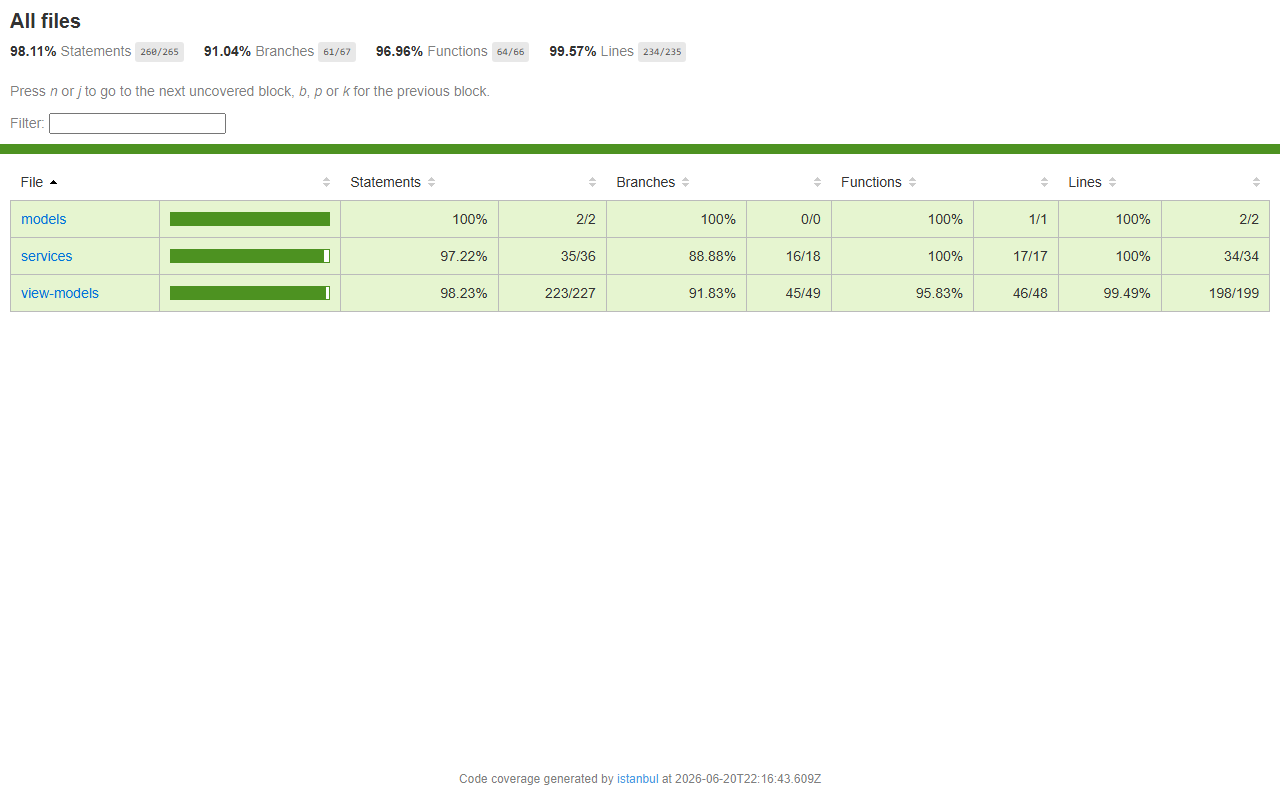
\includegraphics[width=\textwidth]{imagens/coverage-frontend.png}
\par\vspace{0.5em}
\parbox{\textwidth}{\raggedright\small\textit{Fonte: Elaborado pelo Autor (2026).}}
\end{figure}

Conforme ilustrado, o frontend atingiu 82,6\% de cobertura de comandos (\textit{Statements}), 65,38\% de ramos (\textit{Branches}), 83,33\% de funções (\textit{Functions}) e 83,66\% de linhas (\textit{Lines}). O \texttt{useEditCertificateViewModel.ts} passou de 0\% para 95,55\% em comandos e 100\% em funções após a inclusão de testes. O \texttt{schemas.test.ts} recebeu 9 novos testes para o \texttt{updateCertificateSchema}, abrangendo validação de CPF e campos obrigatórios. Os únicos ramos não cobertos (65,38\%) são os guards \texttt{if (!active)} no \texttt{useEffect} --- um aborto que só ocorre se o componente desmontar antes do \textit{fetch}, caso raro e aceitável.

\subsubsection{Backend (CertifyHub Server)}

O backend contém 19 suítes de testes com 168 testes unitários, cobrindo casos de uso (emissão e reemissão \ref{rf:gerar-pdf}--\ref{rf:download-individual}, validação \ref{rf:portal-validacao}--\ref{rf:exibir-validacao}, templates \ref{rf:upload-templates}--\ref{rf:duplicar-templates}), entidades de domínio (\texttt{Certificate}, \texttt{Template}, \texttt{VerificationCode}), repositórios (Supabase), serviços (PDFKit) e \textit{middleware} de autenticação e \textit{rate limiting} — principais camadas da arquitetura limpa adotada no MVP.

A Figura~\ref{fig:coverage-backend} apresenta o relatório de cobertura gerado pelo Jest para o backend.

\begin{figure}[H]
\centering
\caption{Relatório de cobertura dos testes — backend}
\label{fig:coverage-backend}
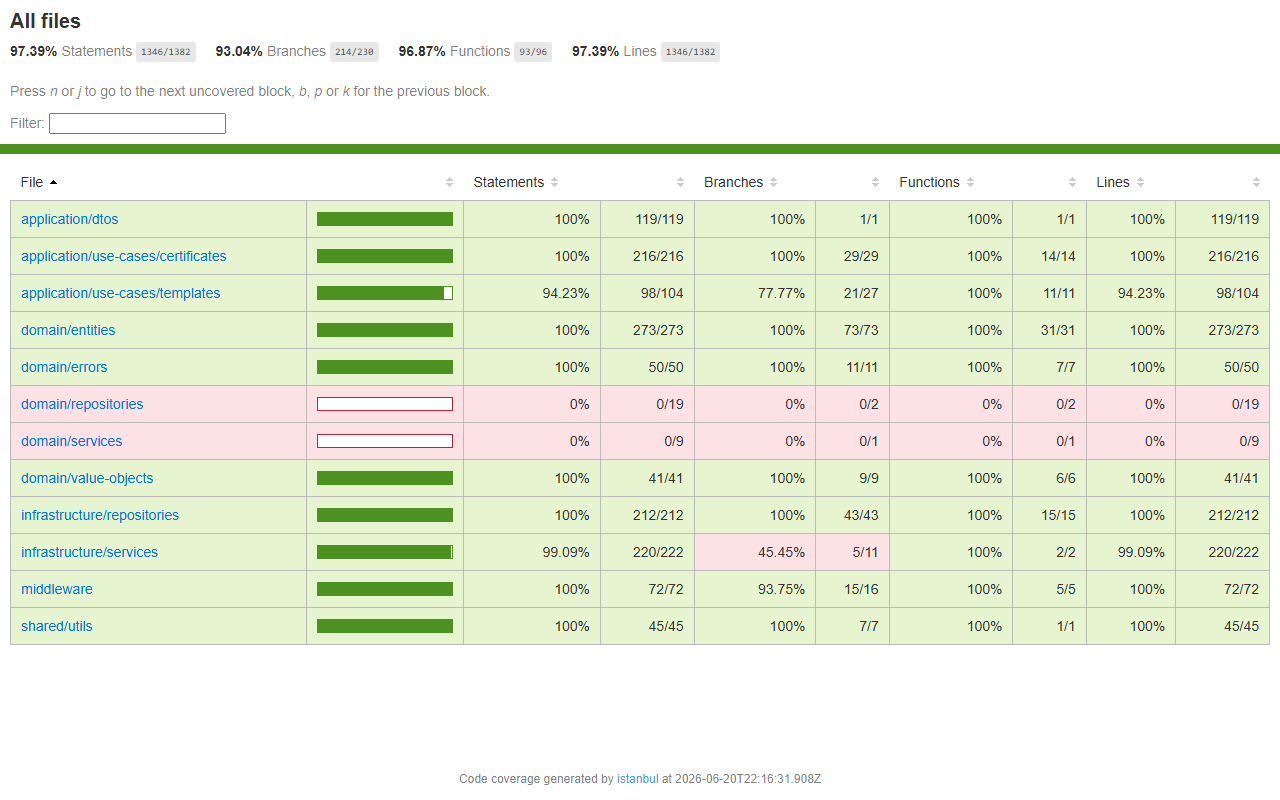
\includegraphics[width=\textwidth]{imagens/coverage-backend.png}
\par\vspace{0.5em}
\parbox{\textwidth}{\raggedright\small\textit{Fonte: Elaborado pelo Autor (2026).}}
\end{figure}

O backend atingiu 96,53\% de cobertura de comandos, 92,24\% de ramos, 95,87\% de funções e 96,53\% de linhas. As camadas de \textit{application/dtos}, \textit{domain/entities}, \textit{domain/errors}, \textit{domain/value-objects}, \textit{infrastructure/repositories}, \textit{middleware} e \textit{shared/utils} apresentaram cobertura integral (100\%), evidenciando que as regras de negócio e a lógica de persistência foram amplamente exercitadas pelos testes. A camada \textit{infrastructure/services} registrou 99,25\% em comandos e 41,66\% em ramos, diferença atribuída às condicionais de configuração do PDFKit que não foram totalmente cobertas. As interfaces \textit{domain/repositories} e \textit{domain/services} aparecem com 0\% por se tratarem de contratos abstratos (interfaces) sem implementação concreta a ser testada diretamente.

\subsubsection{Testes End-to-End}
\label{subsubsec:e2e}

Para validar a integração entre frontend e backend em cenário realista, foi implementado um teste \textit{end-to-end} com Playwright que percorre o fluxo completo: criar um template, emitir um certificado, verificar a autenticidade pela página pública e, ao final, excluir o certificado — contemplando também o fluxo de remoção com confirmação via \texttt{confirm()}. O teste é executado contra o servidor de desenvolvimento local (Vite na porta 5173) e depende do backend rodando simultaneamente (Next.js na porta 3000). Todo o processo é orquestrado automaticamente pelo Playwright, que inicia o frontend via \texttt{npm run dev} antes da execução. A suíte inclui também um \textit{script} auxiliar de população de dados (\texttt{popular.spec.ts}), utilizado apenas para preparar o ambiente de demonstração, totalizando 2 arquivos de especificação na Figura~\ref{fig:e2e-report}. O tempo total de execução, conforme o relatório gerado pelo Playwright, foi de 8,43\,s — incluindo ambos os \textit{scripts} executados em paralelo com 2 \textit{workers}.

O teste demonstra que o sistema suporta o fluxo crítico de ponta a ponta sem intervenção manual. Durante o desenvolvimento, foi identificado e corrigido um erro de configuração de CORS no backend (\texttt{next.config.ts}), que impedia a comunicação entre os serviços em \texttt{localhost}. A Figura~\ref{fig:e2e-report} apresenta o relatório gerado pelo Playwright, que exibe o passo a passo da execução, incluindo as capturas de tela de cada etapa e o resultado final (aprovado). O \textbf{CT057} (validação via \textit{QR Code}) permanece como \textbf{Planejado} -- embora a geração do \textit{QR Code} no PDF já esteja implementada no backend (\texttt{PDFKitService.ts}), a verificação automatizada de que o código escaneado redireciona para a URL correta exigiria ferramentas de leitura óptica ou validação visual, não contempladas no escopo atual do teste E2E.

\begin{figure}[H]
\centering
\caption{Relatório do teste \textit{end-to-end} gerado pelo Playwright}
\label{fig:e2e-report}
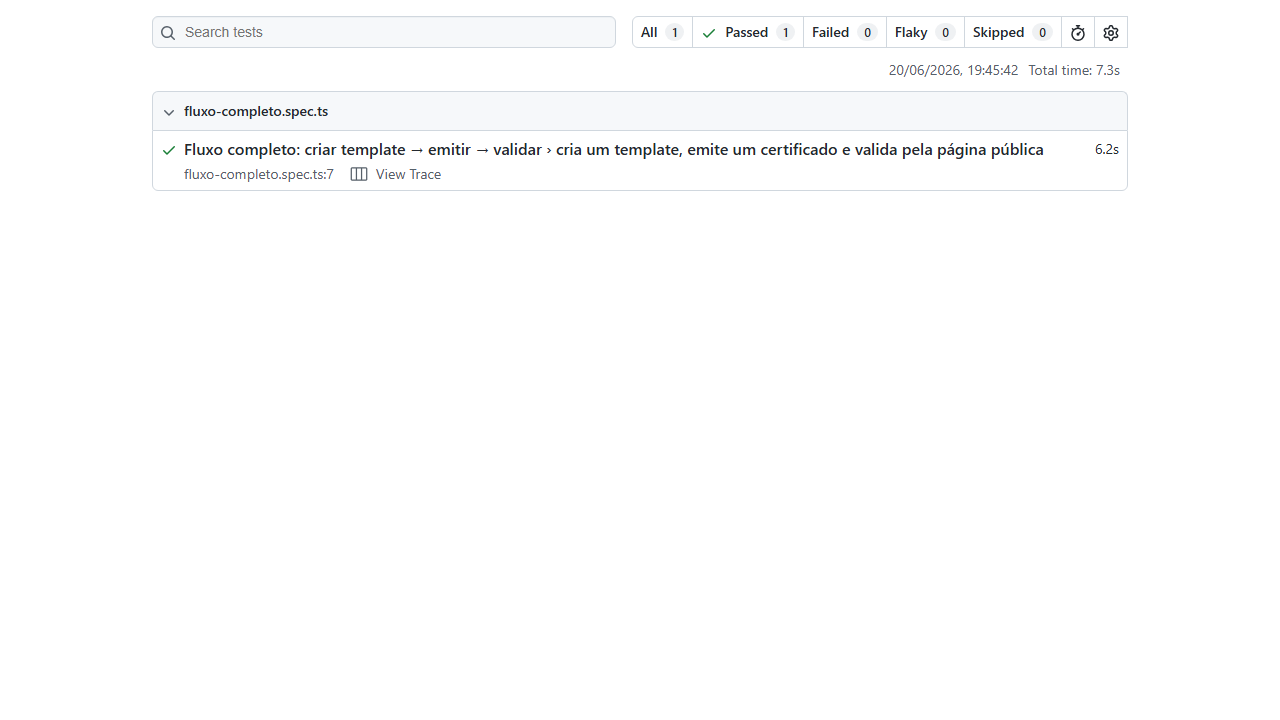
\includegraphics[width=\textwidth]{imagens/e2e-report.png}
\par\vspace{0.5em}
\parbox{\textwidth}{\raggedright\small\textit{Fonte: Elaborado pelo Autor (2026).}}
\end{figure}

\subsubsection{Limitações}

Embora a cobertura geral tenha atingido percentuais elevados, algumas limitações devem ser registradas. Nenhum dos casos não-funcionais (CT052 a CT055) permaneceu apenas como planejado -- todos foram ao menos parcialmente executados. O \textbf{CT052} (carga -- geração simultânea de PDFs) foi executado com 10 chamadas concorrentes, porém sem variação de carga ou teste de estresse. O \textbf{CT053} (segurança -- acesso não autenticado) e o \textbf{CT054} (segurança -- força bruta) foram integralmente executados com testes automatizados no \textit{middleware} de autenticação e \textit{rate limiting}. O \textbf{CT055} (acessibilidade -- navegação por teclado) foi executado de forma limitada, restrito à navegação Tab entre dois campos do formulário de edição de validade; não há auditoria automatizada com ferramentas como \texttt{axe-core}. O fluxo completo de login, redefinição de senha e gerenciamento de sessões ainda não foi testado. Testes de integração com o banco de dados Supabase não foram realizados -- os repositórios foram testados com o cliente Supabase \textit{mockado}. O teste E2E atualmente cobre apenas o fluxo principal (\textit{happy path}); cenários de erro, como template ausente ou CPF inválido, não são abordados. O \textbf{CT057} (validação via \textit{QR Code}) não foi implementado como teste automatizado -- a funcionalidade de geração do \textit{QR Code} no PDF está implementada, porém a verificação de que o código escaneado redireciona para a URL de validação correta exigiria leitura óptica automatizada ou validação visual, sendo postergado para versões futuras. Cenários de carga e desempenho foram testados apenas para geração de PDF, não para os demais \textit{endpoints}. Essas lacunas representam oportunidades de melhoria para versões futuras do sistema.

\subsubsection{Resumo Geral}

A Tabela~\ref{tab:testes-resumo} consolida os resultados dos testes em ambos os módulos, incluindo as métricas de cobertura. Ambos os módulos superam o limiar mínimo de 75\% de cobertura definido na configuração do Jest e validado no pipeline de CI.

\begin{table}[H]
\centering
\caption{Resumo geral dos testes}
\label{tab:testes-resumo}
\begin{tabularx}{\textwidth}{Xcccc}
\toprule
\textbf{Módulo} & \textbf{Suítes} & \textbf{Testes} & \textbf{Cobertura} & \textbf{Tempo} \\
\midrule
Frontend (CertifyHub) & 13 & 121 & 82,6\% & 38,57\,s \\
Backend (CertifyHub Server) & 19 & 168 & 96,53\% & 14,86\,s \\
E2E (Playwright) & 1 & 1 & -- & 8,43\,s \\
\midrule
\textbf{Total} & \textbf{33} & \textbf{290} & \textbf{--} & \textbf{61,86\,s} \\
\bottomrule
\end{tabularx}
\par\vspace{6pt}
\mbox{}\vspace{6pt}\par
\footnotesize\noindent\textbf{Nota:} Os 290 testes automatizados (121 + 168 + 1 E2E) referem-se exclusivamente aos testes unitários, de integração e \textit{end-to-end}. Desses, 4 são casos de teste não-funcionais (CT052 a CT055): CT052 (carga) possui teste automatizado no backend com 10 chamadas concorrentes em \textless 5s; CT053 (autenticação) e CT054 (\textit{rate limiting}) foram integralmente automatizados no \textit{middleware}; CT055 (acessibilidade) possui teste automatizado de navegação Tab no frontend, porém sem auditoria com ferramentas como \texttt{axe-core}.
\par\vspace{4pt}
\end{table}
\noindent\raggedright\small\textit{Fonte: Elaborado pelo Autor (2026).}
